\documentclass[a4paper]{article}
\usepackage[left=3cm, right=3cm, top=2cm, bottom=3cm]{geometry}

\usepackage{setspace}
\usepackage{listings}
\usepackage{authblk}
\usepackage{array}
\usepackage{tabularx}
\usepackage{multirow}
\usepackage[sort&compress]{natbib}
\usepackage[portuguese]{babel}
\usepackage[hidelinks]{hyperref}
\usepackage{xcolor}
\usepackage[inline]{enumitem}
\usepackage{amsmath}
\usepackage{mathtools}

\usepackage{tikz}
\usetikzlibrary{trees}

\usepackage{graphicx}
\graphicspath{ {./images/} }

\newlist{ilist}{enumerate*}{1}
\setlist[ilist]{label=(\arabic*)}

\begin{document}
\title{{\itshape Symbolic Regression}}
\author{Matheus Cândido Teixeira\thanks{matheuscandido2009@gmail.com}}
\affil{Departamento de Ciências da Computação - UFMG}
\maketitle

\section{Introdução}
A regressão simbólica (RS) é utilizada para resolver o problema de \emph{curve
fitting}. Para isso, um conjunto de amostras é fornecido, e o resultado é uma
função que possui o menor erro entre os pontos amostrados e o valor dela nesses
pontos.

Há diversos métodos de aplicar a regressão simbólica~\citep{jin2019}. Uma delas
é utilizando programação genética (GP, do inglês \textit{Genetic
  Programming})~\citep{poli2008}.  A GP é semelhante ao Algoritmo Genético (GA,
do inglês Genetic Algorithm) no que tange os operadores genéticos, pois ambos
definem operadores de inicialização, seleção, cruzamento, mutação e
\textit{fitness}.

Na literatura, há diversas possiveis implementações dos operadores de GP. Por
exemplo, na fase de geração de indivíduos, que podem ser gerados utilizando o
método \textit{full} ou \textit{grow}. No primeiro método, o indivíduo é
complemente gerado, isto é, todos os seus nós são preenchidos, enquanto que no
último, não há essa necessidade. Na prática, é comum haver a combinação dos dois
métodos, denominado \textit{ramped half-and-half}~\citep{poli2008}, onde parte
da população é gerada um dos método e o restante utilizando o outro. A seguir é
apresentado as alternativas comuns para o desenvolvimento de cada operador.

Os operadores de seleção são os mesmos dos utilizados em GA:
\textit{roulette~whell} e \textit{k-tournament}. O primeiro seleciona o
indivíduo com probabilidade proporcional a \textit{fitness} do indivíduo, ou
seja, se a fitness de um indivíduo for \emph{$f_k$} em uma população com $N$
indivíduos, a probabilidade dele ser selecionado é igual a $p(k) =
f_k/\sum_{i=0}^{N}f_i$. O outro método é o \textit{k-tournament}, que amostra
$k$ indivíduos aleatóriamente e seleciona o indivíduo com maior \textit{fitness}
nesse grupo. A diferença entre esses algoritmos está na pressão seletiva imposta
aos indivíduos. Porém \citet{poli2008} informa que o método
\textit{k-Tournament} é o mais comum.

O operador de cruzamento (ou \textit{crossover}) mais comum é denominado troca
de sub-árvore. Esse operador funciona da seguinte maneira: dois indivíduos
($I_1$ e $I_2$, respectivamente) são selecionados da população utilizando o
operador de seleção, após isso, para cada indivíduo, é escolhido um ponto
aleatório ($p_1$ e $p_2$) e um novo indivíduo é gerado pela junção da árvore
$I_1$ sem a sub-árvore com raíz no ponto $p_1$ com a sub-árvore extraida do
$I_2$ com raíz em $p_2$.

No caso do operador de mutação há diversas alternativas, entre elas estam a
mutação de um ponto e mutação de sub-árvore. O primeiro método, percorre todo o
indivíduo muda o gene com uma probabilidade $p_{op}$. O segundo método, seleciona
um ponto aleatório na árvore e, a partir desse ponto, uma sub-árvore é gerada
aleatóriamente. Note que no primeiro método há duas probabilidades envolvidas:
\begin{ilist}
\item a probabilidade de ocorrer mutação ($p_m$) e
\item a probabilidade de haver mutação em cada nó ($p_{op}$), caso o indivíduo
  tenha sido selecionado para mutação.
\end{ilist}

O último operador é o cálculo da \textit{fitness}. Como a regressão simbólica
busca minimizar o erro entre função gerada é os pontos amostrais, é comum
utilizar o erro (a diferença entre o ponto e o resultado da função nesse ponto)
como a forma de mensurar a adequação do indivíduo. Portanto, a \textit{fitness}
pode ser calculada como a somatória do erro absoluto (MAE), somatória do
quadrado do erro (MSE) ou raíz quadrada da somatória do quadrado do erro (RMSE)
entre a função gerado e os pontos amostrais fornecidos, onde as equações são
fornecidas a seguir:
\begin{align*}
  \textrm{MAE} &= \sum_{i}^{N}|y-\hat{y}| \\
  \textrm{MSE} &= \sum_{i}^{N}(y-\hat{y})^2 \\
  \textrm{RMSE} &= \sqrt{\sum_{i}^{N}(y-\hat{y})^2} = \sqrt{\textrm{MSE}}\\
\end{align*}

Outro aspecto importanto em GP é a representação dos indivíduos, que podem ser
representados linearmente ou em árvore. Ambas as representações possuem
vantagens, porém é mais comum a implementação em árvore. Juntamente com a
representação é importante definir os conjuntos de valores que eles podem
assumir. A escolha do conjunto de funções e operadores devem atender a três
restrições: Suficiência, Parcimônia e Fechamento~\footnote{Suficiência significa
que é possível expressar uma solução para o problema utilizando o conjunto de
operadores fornecido. Fechamento significa que os operadores devem suportar
todos os resultados dos demais. Parcimônia significa que o conjunto de
operadores não deve conter elementos desnecessários para representar os
indivíduos.}.

Por exemplo, para uma árvore com um conjunto de funções F:
$\{\sin(\cdot),\cos(\cdot)\}$ , com um conjunto de operadores $S: \{\times, + ,
-, \div\}$, uma possível árvore, cuja expressão é $\sin(ax^2)+\cos(by^2)$, onde
$a$ e $b$ são constantes numéricas e $x$ e $y$ são variáveis independentes, é:


\begin{center}
  \begin{tikzpicture}[level distance=.8cm,
      level 1/.style={sibling distance=4cm},
      level 2/.style={sibling distance=3cm},
      level 3/.style={sibling distance=2cm}]
    \node {+}
    child{node{$\sin$}
      child{node{$\times$}
        child{node{a}}        
        child{node{$\land$}
          child{node{x}}
          child{node{2}}
        }
      }
    }
    child{node{$\cos$}
      child{node{$\times$}
        child{node{b}}        
        child{node{$\land$}
          child{node{y}}
          child{node{2}}
        }
      }
    };  
  \end{tikzpicture}
\end{center}

Neste trabalho, o GP é utilizado para resolver o problema da RS. Os detalhes e
parâmetros da implementação são apresentados nas próximas seções. Para mensurar
a eficiência, o algoritmo é aplicado a 2 dataset, o primeiro é um dataset para
teste, que possui uma versão pura e outra com raídos aleatórios. O outro dataset
é um real e contém 8 colunas de \textit{features} e uma representando a
resposta.

O restante deste relatório é dividido em 3 seções: 
\begin{ilist}
\item A seção de metodologia apresenta os detalhes e escolhas de implementação
  e design de projeto.
\item A seção de experimentos apresenta os resultados obtidos do treinamento
  do algoritmo nos datasets.
\item Por fim, a seção de conclusão analisa os resultados obtidos da seção de
  experimentos.
\end{ilist}

\section{Metodologia} \label{sec:metodologia}
Nesta seção é descrito os datelhes de implementação e as decisões de design
aplicadas neste projeto. A descrição e detalhes são apresentados na ordem:
representação dos indivíduos, métodos de geração de indivíduos, métodos de
seleção, operador de crossover, operador de mutação, operador de reprodução,
eletismo e mecânismos de controle (ou de parada).

\subsection{Reprentação dos indivíduos} \label{subsec:representacao}
A representação dos indivíduos impacta diretamente na performance do sistema e
na expressividade dos invidívuos. Portanto, a princípio é apresentado como o
genótipo do indivíduo é definido e como ele é codificado.


Os indivíduos em GP são representados por árvores sintáticas, que possuem nós e
terminais. Os nós são operadores aritméticos ou funções e os terminais são
constantes ou variáveis. O conjunto de nós e terminais juntos formam o
\textit{primitive set} do GP~\citep{poli2008}. Neste sistema o conjunto de
funções são as funções trigonométricas ($\sin$, $\cos$ e $\tan$) e o logaritmo
com bases diferentes ($\log$ e $\log10$). As constantes são geradas
aleatóriamente utilizando uma distribuição multimodal. A escolha desse método se
deve ao fato que muitas função matemáticas possuem contantes no intervalo $(0,
1]$ e com sinal variado.  As variáveis são geradas aleatóriamente, onde um
  número inteiro no intervalo $(0, N]$, onde $N$ deve ser menor ou igual ao
    número de colunas do dateset menos um, ou seja, se há 10 colunas de
    \textit{features} e uma que representa a variável de resposta, então $N$
    deve ser igual ao número de \textit{features} ou menor.

Outro aspecto importante na representação dos indivíduos é que eles são
geralmente representados por uma estrutura de árvore. A literatura define
diversas estruturas de árvores, como árvores binárias, B-\textit{tree}, entre
outras. Um problema na representação utilizando esses tipos de árvores é a
indireção, que pode afetar a performance do sistema~\citep{faria2013}, portanto,
para evitar os efeitos da indireção de ponteiros, os indivíduos são
representados utilizando \textit{Heaps}, que são árvores especializadas. Nesse
tipo de estrutura, os ponteiro são implicitamente substituidos por indices. O nó
a esquerda está na posição $2n+1$ e $2n + 2$. Outra vantagem no uso de
\textit{Heaps} está no fato dos dados serem armazenados linearmente, o que reduz
os efeitos do \textit{cache miss}, causado por dados espalhados na memória.

O sistema é flexível na escolha da máxima profundidade que um indivíduo
(representado por uma árvore) possui e permite ao usuário especificar qualquer
profundidade aos indivíduos.  Um fator que pode ser vantajoso é que o espaço
ocupado por um indivíduo é determinístico, ou seja, se a profundidade for de
$l$, então a quantidade de nós nessa profundidade é $2^l$.  A quantidade total
de nós que um indivíduo possui é igual a $\sum_{l=0}^{L}2^l=2^{L}-1$, onde $L$ é
a profundidade máxima da árvore. Portanto, para uma população com $N$ indivíduos
e profundidade máxima $L$, há $N\times(2^{L}-1)\times\texttt{sizeof(nó)}$ bytes
ocupados.

Em conclusão, os indivíduos são representados como árvore no ponto de vista
semântico e como vetor contíguo na memória.  Espera-se que com essa estrutura
haja um ganho na performance devido a redução dos efeitos da indireção e por
conseguência de \textit{cache miss}.

\subsection{Operadores de Geração} \label{subsec:generation}

A literatura de define vários operadores de geração de indivíduos, como o método
\textit{Full}, \textit{Grow} e a combinação de ambos, denominado \textit{Ramped
  Half and Half}. O método \textit{Full}, gerada um indivíduo preenchendo todos os
seus nós. O método \textit{Grow}, em contraste com o método anterior, preenche
um usuário não necessariamente preenchendo todos os nós. Por fim, o último método
gera individuos utilizando os dois métodos anteriores, com 50\% de probabilidade
para ambos~\citep{poli2008}.

Nessa implementação, há suporte para os três tipos de geração. O método
\textit{Full} é gerado iterativamente, preenchendo os $L-1$ niveis da árvore do
indívido com funções ou operadores e a última camada com terminais (constantes
ou variáveis).  O método \textit{Grow} é gerado com uma função recursiva, que
escolhe um operador ou função como raíz e utiliza uma função de distribuição
uniforme para decidir se avança ou não mais um nível em cada ramo da árvore,
isto é, o filho à esquerda ou à direita. Já o método \textit{Ramped
  Half-and-Half} utiliza também uma função de distruibuição uniforme para
decidir qual dos dois métodos utilizar.

\subsection{Operadores de Seleção} \label{subsec:selection}

Dois operadores de seleção que são frequentemente utilizados são o
\textit{Roulette Wheel} e o \textit{k-Tournament}. O primeiro método seleciona
algum indivíduo da população com probabilidade proporcional a sua
\textit{fitness}, isto é, $p(i)=f_i/\sum_{k=0}^{N}f_k$. Já o último método
amostra \textit{k} indivíduos aleatoriamente e seleciona o indivíduo que possui
a maior \textit{fitness} dessa amostragem. O método \textit{Tournament} possui
a vantagem de permitir o ajuste da pressão seletiva aplicada, onde valores
menores de $k$ geram baixa pressão seletiva ao passo que grandes valores de $k$
aumentam a pressão seletiva~\citep{Baeck1994}.

Na aplicação desenvolvida é possível utilizar ambos os métodos de seleção. Para
o \textit{k-Tournament} também é possível especificar o valor de \textit{k}.
Essa flexibilidade facilita os testes e a escolha do valor adequado para o
parâmetro, que ajusta a pressão seletiva da seleção e, assim, na interfere na
convergência da população.

\subsection{Operadores de \textit{Crossover}} \label{subsec:crossover}

A operação de \textit{crossover} utiliza o \hyperref[subsec:selection]{operador
  de seleção} para a escolha de dois indivíduos para que eles possam
reproduzir. A reprodução depende de dois fatores: a probabilidade de
\textit{crossover} ($p_c$) e o método de \textit{crossover}.  Uma método comum
para realizar esse evento é denominado troca de sub-árvore, onde duas árvores
são selecionadas utilizando os operadores de seleção e para cada árvore um ponto
é selecionado aleatóriamente. Para uma árvore, o pai, a sub-árvore com raíz no
ponto selecionado é removido e no lugar é inserido a sub-árvore com raíz no
ponto selecionado na outra árvore, a mãe. A escolha do ponto que determina a
raíz da sub-árvore é feaita aleatóriamente, porém , na implementação do
algoritmo, a escolha desses pontos é feita de tal modo que a soma da
profundidade da árvore pai da raíz até o ponto selecionado com a profundidade da
sub-árvore oriunda dá árvore mãe não seja maior de que o comprimento máximo que
um indivíduo pode possuir.

No que tange a implementação, o parâmetro $p_c$ pode assumir qualquer valor no
intervalo $(0, 1)$. A decisão desse parâmetro pode alterar o valor dos
\hyperref[subsec:mutation]{operadores de mutação} ($p_m$) e do
\hyperref[subsec:reproduction]{operador de reprodução} ($p_r$). A forma como a
probabilidade deles pode ser ajustada automaticamente em situações específicas é
descrito na seção \nameref{subsec:smart_par}.

\subsection{Operadores de Mutação} \label{subsec:mutation}

A literatura define os operadores de dois tipos de operadores de mutação:
mutação de sub-árvore e \textit{one-point mutation} (OPM)~\citep{poli2008}. No
primeiro método um ponto é escolhido aleatóriamente na árvore e, a partir desse
ponto, uma sub-árvore é gerada aleatóriamente. No algoritmo implementado, o
método de geração da sub-árvore é o mesmo empregado no método \textit{grow} de
geração (veja Seção \ref{subsec:generation}). O outro método de mutação é o
OPM. Esse método é aplicado sobre todos os nós e terminais da árvore do
indivíduo, onde há a probabilidade de $p_op$ de haver mutação nesse nó. A
mutação em um nó específico ocorre alterando o elemento contido nele por outro
da mesma classe, por exemplo, em um nó contendo a função $\sin$, a OPM pode
alterá-lo para $\tan$, ou seja, manteve a classe (uma função), porém alterou o
elemento contido no nó.

Na implementação, ambos os métodos possuem igual probabilidade de serem
empregados (50\%-50\%, respectivamente), porém no caso do OPM a probabilidade de
mutação de cada nós é especificado separadamente e é possível controlar o valor
dessa probabilidade através da constante $p_op$, que controla a probabilidade de
OPM.

\subsection{Operador de Reprodução} \label{subsec:reproduction}

Quando a probabilidade de \textit{crossover} e de mutação somadas é menor do que
100\%, algebricamente expresso por $p_c + p_m < 1$, entra em ação o operador
de reprodução, que basicamente seleciona indivíduos da população utilizando
o operador de seleção selecionado até que a próxima geração atinja o tamanho
máximo da população.

Esse parâmetro pode ser ajustado na aplicação através do parâmetro $p_r$, e,
dessa forma, os operadores de mutação ($p_m$) e de \textit{crossover} ($p_c$)
são ajustados automaticamente.

\subsection{Eletismo}

Após a geração da próxima geração de indivíduos há duas possibilidades:
descartar a população anterior ou manter os indivíduos da população anterior
com a nova população e selecionar os que possuem maior \textit{fitness} em ambas
as populações. Essa última abordagem é denominada eletismo.

O sistema desenvolvido permite que a aplicação do eletismo seja controlado pelo
parâmetro $E$, que indica se deve ou não ocorrer eletismo.

\subsection{\textit{Fitness}}

A \textit{Fitness} determina o quão adaptado um indivíduo está e é utilizada
para comparação entre os indivíduos. A função para calcular a \textit{fitness}
está relacionada ao problema, e, no caso da RS, algumas formas de mensurar a
\textit{fitness} de um indivíduos são o erro médio absoluto (MSA), o error médio
quadrado (MSE) e a raiz do erro médio quadrado (RMSE). Independente da métrica
utilizada para calcular a \textit{fitness}, o objetivo é minimizar o erro.

Na implementação desenvolvida todas as três métricas descritas estão disponíveis
e fica a critério do usuário a escolha de qual métrica de erro utilizar.

\subsection{Ajuste Inteligente de Parâmetros}\label{subsec:smart_par}

As probabilidades de \textit{crossover} ($p_c$), de mutação ($p_m$) e de
reprodução ($p_r$) estão relacionadas através da seguinte equação:
\begin{equation} \label{eq:prob_stability}
  p_c + p_m + p_r = 1
\end{equation}
Geralmente, é comum atribuir valores altos para $p_c$ e mais baixos $p_m$, porém
quando eles não somam a 1, o operador de reprodução $p_r$ é atribuido ao
complemento, de tal forma que a equação \ref{eq:prob_stability} é satisfeita.

Outra forma de controle ocorre quando o usuário atribui um valor para $p_r$,
neste caso, os valores de $p_c$ e $p_m$ são ajustado para que a soma deles
resulte em $1-p_r$. Quando isso ocorre, a proporção relativa entre eles é
mantida, isto é:

\noindent\begin{minipage}{.5\linewidth}
  \begin{equation*}
    p_c = \frac{p_c}{p_c+p_m}\times (1-p_r)  
  \end{equation*}
\end{minipage}
\begin{minipage}{.5\linewidth}
  \begin{equation*}
    p_m = \frac{p_m}{p_c+p_m}\times (1-p_r)  
  \end{equation*}
\end{minipage}

\subsection{Ambiente para Testes}

Devido ao fato da GP tomar decisões aleatóriamente, o resultado pode variar
entre execuções. Para alcançar um grau de confiança nos resultados obtidos, é
necessário repetir os testes diversas vezes. Para isso, o sistema implementado
possui suporte para testes.

Para testar os alguns parâmetro o usuário deve fornecer um arquivo
\texttt{*.csv}, onde cada linha deve conter uma lista de números inteiros que
são utilizados como \textit{seeds} para o geradores de números aleatórios. O
gerador utilizado na implementação é o \texttt{32-bit Mersenne Twister}. Os
testes são repetidos para cada linha contida no arquivo contendo as
\textit{seeds}.

\subsection{Desempenho}

Conforme mensionado nas seções anteriores, as escolhas da representação dos
indivíduos foi feita tendo em vista a performance do sistema. Um fator a ser
explorado é a performance do sistema com a introdução de paralelismo.

\subsection{Compilação}
A implementação do algoritmo foi feito em \texttt{C++}. A compilação pode ser
complexa devido a quantidade de depências em bibliotecas para leitura de
arquivos \texttt{*.csv} e \textit{parser} dos argumentos. Para contornar essa
complexidade, o CMake foi utilizado para gerar o projeto de modo que o sistema
utilize o compilador \texttt{C++} disponível no sistema. Os comandos necessários
para compilar e executar o programa utilizando o Linux pode ser visto no
\hyperref[lst:code]{Código~\ref*{lst:code}}.

\begin{lstlisting}[language=bash, caption={Comandos para compilar utilizando o Linux},
    label={lst:code}, frame=shadowbox, frameround=fttt]
  mkdir bin 
  cd bin    
  cmake ..  
  cmake --build .  
  cd src           
  ./sreg [parameters]
                    
\end{lstlisting}

\section{Experimentos}
Nesta seção é apresentado resultados dos experimentos realizados. Os resultados
apresentados são estatísticas geradas a partir da execução dos parâmetros
mantidos fixos e alterando apenas as \textit{seeds} do gerador
pseudo-aleatório. São fornecidos para o teste 31 sementes, cada uma contendo 20
números inteiros gerados aleatóriamente.  Ao aplicar o mesmo conjunto de
sementes, os resultados devem ser reproduzíveis.

\subsection{Dataset Experiamental}
Este dataset possui uma versão sem ruído e uma versão ruidosa. O algoritmo será
aplicado em ambas as versões.

O primeiro teste tem o objetivo de identificar qual o tamanho da população que
atinge o menor valor de \textit{fitness} em média. Para isso, o tamanho da
população é variado e os demais parâmetros são mantidos constantes. As
estatísticas da repetição do algoritmo para cada tamanho de população é
apresentado na \hyperref[tbl:default_param]{Tabela~\ref*{tbl:default_param}},
onde cada coluna representa uma informação da população e cada linha representa
estatísticas dos resultadas da repetição do algoritmo para diferentes
\textit{seeds}.

\noindent
\begin{table}
  \center
  \caption{Parâmetros \textit{default}}
  \label{tbl:default_param}
  \begin{tabular}{| c | c | c | c | c | c | c | c | c | c |}
    \hline
    \# Vars & MaxG & MG & MD & MS & $p_c$ & $p_m$ & ME & T & E \\
    \hline
    1 & 40 & \textit{Ramped HH} & 7 & 3-Tournament & 0.9 & 0.05 & MAE & $10^{-9}$ & 0 \\
    \hline
  \end{tabular}
  \begin{minipage}{.9\textwidth}{\center \setstretch{0.1} \footnotesize \# Vars indica a quantidade de
      váriaveis. MaxG é o limite de gerações. MG é método de geração da
      população. MD é a profundidade máxima dos indivíduos. MS é o método de
      seleção.  $p_c$ e $p_m$ são a probabilidade de crossover e mutação,
      repectivamente. ME é a métrica de erro, T é o threshold mínimo e E indica
      a presença de eletismo.}\end{minipage}
\end{table}

Os valores testados da população são 50, 100, 300 e 500 indivíduos. Os resultados
são apresentados na \hyperref[tbl:result_pop]{Tabela~\ref*{tbl:result_pop}}.
As estatísticas coletadas são a quantidade de indivíduos únicos, a quantidade de
indíduos melhores que a mediana da geração passada, a menor, a maior, a mediana,
o desvio padrão e a média da \textit{fitness} da população após as atingir as
40 gerações. Como o teste foi repetido 31 vezes com sementes diferentes, as
estatísticas da população final de todas elas são sumarizadas. Os resultados
indicam que com a população de 500 indivíduos a média da \textit{fitness} mínima
da população é de 0.19, portanto, os próximos experimentos serão realizados
mantendo-se a população com 500 indivíduos.

\noindent
\begin{table}[h!]
  \center
  \caption{Resultado do tamanho da população}
  \label{tbl:result_pop}
  \begin{tabular}{| c | c | c | c | c | c | c | c | c |}
    \hline
    &  \# U & \# M & min. & max. & median. & stddev & avg. & Pop. \\ \hline \hline
    avg. & 4.93 & 2.96 & 0.195 & 925.24 & 0.199 & 129.83 & 18.93 &  \multirow{5}{1.5cm}{50} \\ \cline{1-8}
    stddev & 6.9 & 8.002 & 0.035 & 3227.92 & 0.015 & 451.81 & 64.51 & \\ \cline{1-8}
    CV & 1.39 & 2.69 & 0.179 & 3.48 & 0.076 & 3.479 & 3.408 & \\ \cline{1-8}
    max. & 42 & 30 & 0.21 & 16756.27 & 0.21 & 2345.84 & 335.39 & \\ \cline{1-8}
    min. & 3 & 0 & 0.01 & 0.47 & 0.12 & 0.05 & 0.21 & \\ \hline \hline
    avg. & 7.03 & 3.6129 & 0.199 & 17006.21 & 0.201 & 1692.58 & 170.83 & \multirow{5}{1.5cm}{100} \\ \cline{1-8}
    stddev & 0.83 & 11.03 & 0.006 & 58480.12 & 0.005 & 5818.47 & 585.48 & \\ \cline{1-8}
    CV & 0.118 & 3.05 & 0.03 & 3.44 & 0.028 & 3.44 & 3.43 & \\ \cline{1-8}
    max. & 10 & 54 & 0.21 & 240038.24 & 0.21 & 23883.07 & 2404.89  & \\ \cline{1-8}
    min. & 6 & 0 & 0.18 & 1.568724 & 0.19 & 0.25 & 0.26 & \\ \hline \hline
    avg. & 19.29 & 14.03 & 0.20 & 19350.68 & 0.20 & 1128.70 & 69.31 & \multirow{5}{1.5cm}{300} \\ \cline{1-8}
    stddev & 6.83 & 30.98 & 0.01 & 55837.68 & 0 & 3219.99 & 188.27 & \\ \cline{1-8}
    CV & 0.35 & 2.21 & 0.03 & 2.89 & 0.02 & 2.85 & 2.72 & \\ \cline{1-8}
    max. & 50.00 & 115.00 & 0.20 & 293033.57 & 0.21 & 16889.95 & 981.34 & \\ \cline{1-8}
    min. & 16.00 & 0.00 & 0.17 & 11.10 & 0.20 & 0.70 & 0.30 & \\ \hline \hline
    avg. & 43.52 & 77.61 & 0.19 & 281293.46 & 0.20 & 12618.11 & 576.70 & \multirow{5}{1.5cm}{500} \\ \cline{1-8}
    stddev & 55.94 & 76.42 & 0.03 & 1080461.83 & 0.01 & 48259.57 & 2159.41 & \\ \cline{1-8}
    CV & 1.29 & 0.98 & 0.19 & 3.84 & 0.03 & 3.82 & 3.74 & \\ \cline{1-8}
    max. & 306.00 & 218.00 & 0.20 & 5960136.66 & 0.21 & 266278.53 & 11925.03 & \\ \cline{1-8}
    min. & 26.00 & 0.00 & 0.01 & 16.40 & 0.20 & 1.04 & 0.34 & \\ \hline
  \end{tabular}
  \begin{minipage}{0.9\textwidth}
    {\center \footnotesize
      \# U: quantidade de indivíduos únicos. \# M: quantidade de indivíduos melhores
      que a mediana da população anterior. min.: Fitness mínima atingida. max.:
      Fitness máxima atingida. median.: mediana da Fitness da população final.
      stddev: Desvio Padrão da Fitness da população final. avg.: Média aritmética.
      Pop.: Tamanho da população.
    }
  \end{minipage}
\end{table}

O próximo experimento é do efeito das probabilidade de mutação e
\textit{crossover}.  Como o teste anterior manteve os parâmetros de $p_c=0.9$ e
de $p_m=0.05$, os próximos experimentos verificam o efeito de aumentar a
probabilidade de mutação e , por consequência, diminuir a probabilidade de
\textit{crossover}.

\begin{table}
  \center
  \caption{Variação da probabilidade de crossover e mutação}
  \label{tbl:var_cross_mut}
  \begin{tabular}{| c | c | c | c | c | c | c | c | c |}
    \hline
    &  \# U & \# M & min. & max. & median. & stddev & avg. & $p_c$/$p_m$. \\ \hline
    avg.    & 274.35 & 130.71 & 0.13 & 1793669.61 & 0.20 & 81221.52 & 3873.49 & \multirow{5}{1.5cm}{$p_c=0.6$\\$p_m=0.3$} \\ \cline{1-8}
    stddev. & 131.73 & 25.82 & 0.08 & 6382322.66 & 0.03 & 284986.57 & 12753.39 & \\ \cline{1-8}
    CV      & 0.48 & 0.20 & 0.63 & 3.56 & 0.14 & 3.51 & 3.29 & \\ \cline{1-8}
    max.    & 468.00 & 174.00 & 0.20 & 33708402.01 & 0.21 & 1505976.37 & 67438.93 & \\ \cline{1-8}
    min.    & 156.00 & 64.00 & 0.00 & 314.24 & 0.08 & 19.12 & 2.13 & \\ \hline \hline
    avg.    & 176.19 & 161.68 & 0.16 & 608201.55 & 0.20 & 27274.88 & 1293.95 & \multirow{5}{1.5cm}{$p_c=0.7$\\$p_m=0.2$} \\ \cline{1-8}
    stddev  & 123.60 & 49.49 & 0.06 & 1590846.25 & 0.03 & 71090.51 & 3294.17 & \\ \cline{1-8}
    CV      & 0.70 & 0.31 & 0.38 & 2.62 & 0.17 & 2.61 & 2.55 & \\ \cline{1-8}
    max.    & 467.00 & 203.00 & 0.20 & 8429830.05 & 0.21 & 376746.76 & 17498.51 & \\ \cline{1-8}
    min.    & 102.00 & 0.00 & 0.00 & 429.51 & 0.03 & 19.85 & 2.32 & \\ \hline \hline
    avg.    & 91.32 & 202.90 & 0.19 & 6679069.20 & 0.21 & 299038.87 & 13859.07 & \multirow{5}{1.5cm}{$p_c=0.85$\\$p_m=0.15$} \\ \cline{1-8}
    stddev  & 72.92 & 73.82 & 0.03 & 28313559.15 & 0.01 & 1265314.09 & 57887.15 & \\ \cline{1-8}
    CV      & 0.80 & 0.36 & 0.17 & 4.24 & 0.03 & 4.23 & 4.18 & \\ \cline{1-8}
    max.    & 484.00 & 252.00 & 0.20 & 157549013.24 & 0.21 & 7039707.91 & 321514.74 & \\ \cline{1-8}
    min.    & 75.00 & 0.00 & 0.02 & 628.67 & 0.19 & 36.60 & 4.35 & \\ \hline
  \end{tabular}
    \begin{minipage}{0.9\textwidth}
    {\center \footnotesize
      Mesmos que da \hyperref[tbl:result_pop]{Tabela~\ref*{tbl:result_pop}}.
      $p_c$: Probabilidade de crossover. $p_m$: Probabilidade de mutação.
    }
  \end{minipage}
\end{table}

Com a variação da probabilidade é possível concluir a partir da
\hyperref[tbl:var_cross_mut]{Tabela~\ref*{tbl:var_cross_mut}} que o algoritmo
atinge a menor \textit{fitness} em média quando a probabilidade de crossover é
menor.  A menor \textit{fitness} média é de 0.13 com $p_c = 0.6$ e $ p_m = 0.3
$, porém a quantidade de indivíduos gerados que são melhores do que a mediana da
população anterior é maior para o último caso, onde $p_c = 0.85$ e $ p_m =
0.15$. Para os próximos experimentos o valor de $p_c = 0.6$ e $ p_m = 0.3$ serão
fixados.

Outro característica a ser testado é tamanho do torneio, isto é, o parâmetro k
do método de seleção \textit{Tournament}. Os teste anteriores foram realizados
com o parâmetro k fixo e com valor 3. Os demais testes modificam o valor de k
para 5, 7 e 10. Os resultados estão presentes na
\hyperref[tbl:var_k]{Tabela~\ref*{tbl:var_k}}. Os resultados indicam que o valor
de $k=5$ são os que resultam no menor valor de \textit{fitness} em média. Para o
último experimento o tamanho do torneio é fixado em $k=5$.


\begin{table}
  \centering
  \caption{Variação do parâmetro k}
  \label{tbl:var_k}
  \begin{tabularx}{1\textwidth}{| X | X | X | X | X | X | X | X | X |}
    \hline
    &  \# U & \# M & min. & max. & median. & stddev & avg. & $k$ \\ \hline \hline
avg. & 299.19 & 158.16 & 0.10 & 360372.62 & 0.21 & 16253.90 & 758.62 & \multirow{5}{1.5cm}{$k=5$} \\ \cline{1-8}
stddev & 107.66 & 19.55 & 0.08 & 1767685.76 & 0.10 & 78952.58 & 3532.77 & \\ \cline{1-8}
CV & 0.36 & 0.12 & 0.81 & 4.91 & 0.49 & 4.86 & 4.66 & \\ \cline{1-8}
max. & 464.00 & 209.00 & 0.20 & 9867700.84 & 0.44 & 440855.16 & 19742.83 & \\ \cline{1-8}
min. & 145.00 & 132.00 & 0.00 & 74.91 & 0.03 & 4.87 & 0.89 & \\ \hline \hline
avg. & 265.87 & 154.23 & 0.11 & 141705.79 & 0.23 & 6368.16 & 303.79 & \multirow{5}{1.5cm}{$k=7$} \\ \cline{1-8}
stddev & 95.11 & 12.26 & 0.07 & 331306.45 & 0.10 & 14808.40 & 675.54 & \\ \cline{1-8}
CV & 0.36 & 0.08 & 0.59 & 2.34 & 0.43 & 2.33 & 2.22 & \\ \cline{1-8}
max. & 448.00 & 183.00 & 0.20 & 1400507.65 & 0.47 & 62569.32 & 2853.22 & \\ \cline{1-8}
min. & 144.00 & 128.00 & 0.00 & 27.26 & 0.04 & 1.86 & 0.54 & \\ \hline \hline
avg. & 218.68 & 148.97 & 0.12 & 8627.45 & 0.25 & 418.71 & 28.16 & \multirow{5}{1.5cm}{$k=10$}\\ \cline{1-8}
stddev & 73.40 & 32.59 & 0.06 & 20553.19 & 0.11 & 952.17 & 57.26 & \\ \cline{1-8}
CV. & 0.34 & 0.22 & 0.45 & 2.38 & 0.46 & 2.27 & 2.03 & \\ \cline{1-8}
max. & 358.00 & 199.00 & 0.18 & 99365.38 & 0.57 & 4597.18 & 270.40 & \\ \cline{1-8}
min. & 129.00 & 0.00 & 0.00 & 50.11 & 0.12 & 4.11 & 1.04 & \\ \hline 
  \end{tabularx}
  \begin{minipage}{0.9\textwidth}
    {\center \footnotesize
      Mesmos que da \hyperref[tbl:result_pop]{Tabela~\ref*{tbl:result_pop}}.
      $k$ é o parâmetro do método de seleção \textit{Tournament}.
    }
  \end{minipage}
  
\end{table}

Por fim, o último parâmetro experimentado é como a presença do eletismo. Os
teste anteriores foram realizados sem eletismo e o próximo experimento é
realizado com o eletismo ativado. Os resultados estão apresentados na
\hyperref[tbl:var_eletism]{Tabela~\ref*{tbl:var_eletism}}. Comparando os resultados
da presença ou ausência de eletimos. Os resultados indicam que a ausência de
eletismo possui o valor da \textit{fitness} menor do que quando ativado. Porém,
outro aspectivo é a diferença no valor máximo da \textit{fitness} entre eles.
Quando o eletismo está ativo, o melhor e o pior indivíduo não estão tão distantes
quando se comparado com os indivíduos gerados com o eletismo desativado.

\begin{table}
  \center
  \caption{Efeitos do eletismo}
  \label{tbl:var_eletism}
  \begin{tabular}{| c | c | c | c | c | c | c | c | c |}
    \hline
    &  \# U & \# M & min. & max. & median. & stddev & avg. & E \\ \hline \hline
avg. & 299.19 & 158.16 & 0.10 & 360372.62 & 0.21 & 16253.90 & 758.62 & \multirow{5}{1.5cm}{0} \\ \cline{1-8}
stddev & 107.66 & 19.55 & 0.08 & 1767685.76 & 0.10 & 78952.58 & 3532.77 & \\ \cline{1-8}
CV & 0.36 & 0.12 & 0.81 & 4.91 & 0.49 & 4.86 & 4.66 & \\ \cline{1-8}
max. & 464.00 & 209.00 & 0.20 & 9867700.84 & 0.44 & 440855.16 & 19742.83 & \\ \cline{1-8}
min. & 145.00 & 132.00 & 0.00 & 74.91 & 0.03 & 4.87 & 0.89 & \\ \hline \hline
avg. & 13.45 & 28.10 & 0.12 & 0.13 & 0.13 & 0.00 & 0.13 & \multirow{5}{1.5cm}{1} \\ \cline{1-8}
stddev & 36.93 & 39.89 & 0.06 & 0.05 & 0.05 & 0.00 & 0.05 & \\ \cline{1-8}
CV. & 2.75 & 1.42 & 0.47 & 0.42 & 0.42 & 2.72 & 0.43 & \\ \cline{1-8}
max. & 207.00 & 172.00 & 0.18 & 0.18 & 0.18 & 0.02 & 0.18 & \\ \cline{1-8}
min. & 1.00 & 0.00 & 0.00 & 0.00 & 0.00 & 0.00 & 0.00 & \\ \hline 
  \end{tabular}
    \begin{minipage}{0.9\textwidth}
    {\center \footnotesize
      Mesmos que da \hyperref[tbl:result_pop]{Tabela~\ref*{tbl:result_pop}}.
      E indica a presença ou ausência de eletismo.
    }
  \end{minipage}
\end{table}

Através dos experimentos realizados, obteve-se que a maior população (500
indivíduos), com maior probabilidade de mutação ($p_c=0.6$ e $p_m=0.3$), com o
parâmetro k do método de seleção \textit{k-Tournament} com 1\% do tamanho da
população ($k=5$) e sem eletismo, atingem o menor valor de \textit{fitness}
entre todos os experimentos conduzidos. Para verificar a robustez do algoritmo
os parâmetros obtidos são também aplicados para o dataset que contém ruídos.

Os resultados apresentados na
\hyperref[tbl:noise_dataset]{Tabela~\ref*{tbl:noise_dataset}} são semelhantes ao
resultados obtidos sem a presença de ruído, conforme pode ser observado na
\hyperref[tbl:var_eletism]{Tabela~\ref*{tbl:var_eletism}}. O que indica que o
modelo criado é capaz de gerar uma função mesmo na presença de ruído.

\begin{table}
  \center
  \caption{Resultados da aplicação no dataset com ruídos}
  \label{tbl:noise_dataset}
  \begin{tabular}{| c | c | c | c | c | c | c | c |}
    \hline
    &  \# U & \# M & min. & max. & median. & stddev & avg. \\ \hline 
avg. & 299.19 & 158.16 & 0.10 & 360372.62 & 0.21 & 16253.90 & 758.62 \\ \hline 
stddev & 107.66 & 19.55 & 0.08 & 1767685.76 & 0.10 & 78952.58 & 3532.77 \\ \hline 
CV & 0.36 & 0.12 & 0.81 & 4.91 & 0.49 & 4.86 & 4.66 \\ \hline 
max. & 464.00 & 209.00 & 0.20 & 9867700.84 & 0.44 & 440855.16 & 19742.83 \\ \hline 
min. & 145.00 & 132.00 & 0.00 & 74.91 & 0.03 & 4.87 & 0.8 \\ \hline
  \end{tabular}
  \begin{minipage}{0.7\textwidth}
    {\center \footnotesize
      Mesmos que da \hyperref[tbl:result_pop]{Tabela~\ref*{tbl:result_pop}}.
    }
  \end{minipage}
\end{table}

\subsection{Dataset Real}
Neste experimento, o sistema é testado com um dataset real. Este dataset contêm
9 colunas. Portanto, a regressão utiliza até 8 diferentes variáveis. A metodologia
é a mesma empregada para no dataset artificial:
\begin{ilist}
\item identificar o tamanho da população
\item identificar a profundidade da árvore
\item identificar o tamanho do torneio (k)
  \item identificar os melhores valores de $p_c$ e $p_m$
\end{ilist}.

Para encontrar os melhores valores de cada parâmetro os demais devem ser fixados.
Os valores iniciais de cada parâmetro são: \textit{Ramped Half-and-Half} como
método de geração, \textit{5-Tournament} como método de seleção, o limite de
gerações é 60, a profundidade da árvore é 7, a probabilidade de crossover e de
mutação são $p_c=0.6$ e $p_m=0.3$, respectivamente.

A princípio, para identificar o tamanho da população os seguintes tamanhos serão
avaliados: 600, 800 e 1200. A \hyperref[fig:var_pop]{Figura~\ref*{fig:var_pop}}
apresenta o valor da menor \textit{fitness} de cada geração para os três tamanhos
de população. O valor final da \textit{fitness} na última geração foi de 5.76
para a população com 800 indivíduos, portanto, este valor é mantido para os
demais experimentos.


O segundo parâmetro a verificar é a profundidade máxima da árvore. Os valores
testados são: 6, 7, 8 e 9. Os valores que a menor \textit{fitness} assume ao
longo das gerações para cada profundidade pode ser visto na
\hyperref[fig:var_d]{Figura~\ref*{fig:var_d}}. Os resultados indicam que a menor
\textit{fitness} é alcançada quando o tamanho da árvore é igual a 8, onde o
valor na última geração é igual a $5.5796$. Quando a profundidade os valores que
\textit{fitness} os indivíduos com profundidade 6, 7 ou 9 assumem são $8.6567$,
$8.7384$ e $6.7258$, respectivamente, indicando que a profundidade igual a 8 é
um ponto de mínimo. Para os próximos teste a profundidade é fixada em 8.


O terceiro parâmetro testado é o tamanho do torneio, ou seja, o valor de $k$.
Os valores testados foram: 8, 10, 12 e 15. Os valores da menor \textit{fitness}
para cada geração para os valores testados podem ser vistos na
\hyperref[fig:var_k]{Figura~\ref*{fig:var_k}}.  Os resultados indicam que o
menor valor é atingindo quando k=8, onde o valor da \textit{fitness} atinge
$5.5796$ ao longo das 60 gerações. Os próximos testes são realizados mantendo-se
o valor de k fixo e igual a 8.

O quarto parâmetro verificado é a probabilidade de \textit{crossover}. Os
valores testados são: $p_c=0.6$, $p_c=0.7$ e $p_c=0.8$. A
\hyperref[fig:var_pc]{Figura~\ref*{fig:var_pc}} mostram os valores da menor
\textit{fitness} em cada geração para cada valor de probabilidade verificado.  O
menor valor atingido em 60 gerações foi $6.1097$ para a população gerada com
$p_c=0.6$. Pelo fato da probabilidade \textit{crossover} estar baixa leva a
probabilidade de recombinação e mutação a estar mais elevada. Esses dois
operadores podem aumentar o \textit{exploration} e \textit{explotation}, pois a
recombinação seleciona os invidíduos mais bem adaptados da população anterior
(\textit{explotation}), já a mutação faz com que novas soluções do espaço de
soluções sejam experimentadas (\textit{exploration}). Essa combinação de
probabilidades de \textit{crossover}, mutação e recombinação são os responsáveis
por atingirem a menor \textit{fitness}. Para o próximo experimento, o valor de
$p_c$ é mantido fixo em $p_c=0.6$.

Para determinar o efeito da mutação e da recombinação, o último teste é variar o
valor de $p_m$. Os valores experimentados são: $p_m=0.1$, $p_m=0.15$,
$p_m=0.20$, $p_m=0.25$ e $p_m=0.30$. Os valores da menor \textit{fitness} de
cada geração para a população gerada com os valores de $p_m$ variados podem ser
vistos na \hyperref[fig:var_pm]{Figura~\ref*{fig:var_pm}}. Os resultados que o
menor valor atingido ocorre quando $p_m=0.30$, onde o valor da \textit{fitness}
é igual a $5.57966$. Isso prova que a mutação tem impacto mais significativo do
que a recombinação, ou seja, neste caso o \textit{exploration} é mais importante
do que o \textit{explotation}.

\begin{figure}[h!]
  \begin{minipage}{0.5\textwidth}
    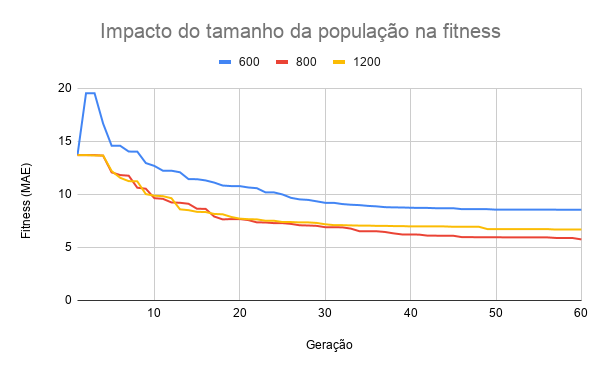
\includegraphics[width=\textwidth]{var_pop}
    \caption{Variação do tamanho da população}
    \label{fig:var_pop}
  \end{minipage}
  \begin{minipage}{0.5\textwidth}
    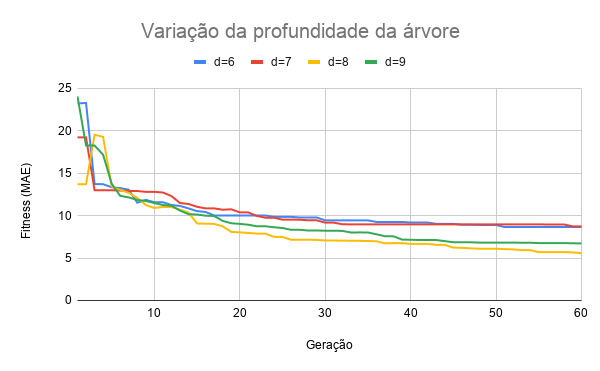
\includegraphics[width=\textwidth]{var_d}
    \caption{Variação da profundidade da árvore}
    \label{fig:var_d}
  \end{minipage}
  \begin{minipage}{0.5\textwidth}
    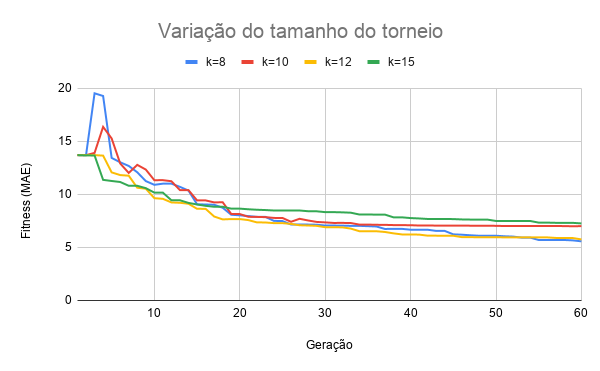
\includegraphics[width=\textwidth]{var_k}
    \caption{Variação do tamanho do torneio}
    \label{fig:var_k}
  \end{minipage}
  \begin{minipage}{0.5\textwidth}
    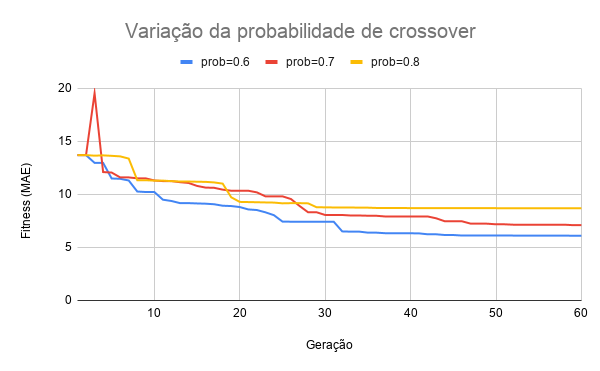
\includegraphics[width=\textwidth]{var_pc}
    \caption{Variação da probabilidade de \textit{crossover}}
    \label{fig:var_pc}
  \end{minipage}
\end{figure}
\begin{figure}[h!]
  \begin{minipage}{0.5\textwidth}
    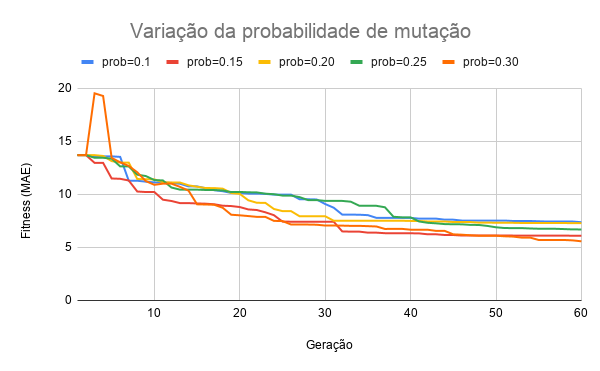
\includegraphics[width=\textwidth]{var_pm}
    \caption{Variação da probabilidade de mutação}
    \label{fig:var_pm}
  \end{minipage}
\end{figure}
\newpage
\section{Conclusão}
Os resultados obtidos indicam a importância entre o balanceamento dos diversos
parâmetros do GP. A probabilidade de mutação, $p_m$, tem grande impacto no valor
mínimo da \textit{fitness}, devido a exploração do espaço de soluções. Outro
fator importante é o tamanho da árvore, pois quando mais complexo os dados,
maior deve ser a profundidade da árvore para obter maior expressividade dos
indivíduos.

Outro aspacto à ser estudado é o tamanho da \textit{fitness}, $5.57966$. Se
comparado com a média do label do dataset \texttt{concrete.csv}, que é
$35.81796$, é possível verificar que o erro é aproximadamente 15\% da magnitude
da média, ou seja, muito elevado. 

\newpage
\bibliographystyle{plainnat}
\bibliography{bibliography}
\end{document}
